%%%%%%%%%%%%%%%%%%%%%%%%%%%%%%%%%%%%%%%%%%%%%%%%%%%%%%%%%%%%%%%%%%%%%%%%%%%%%%%%
% Front matter
%%%%%%%%%%%%%%%%%%%%%%%%%%%%%%%%%%%%%%%%%%%%%%%%%%%%%%%%%%%%%%%%%%%%%%%%%%%%%%%%

\title{pdp: An R Package for Constructing Partial Dependence Plots}
\author{by Brandon M. Greenwell}

\maketitle

\abstract{
Complex nonparametric models---like neural networks, random forests, and support vector machines---are more common than ever in predictive analytics, especially when dealing with large observational databases that don't adhere to the strict assumptions imposed by traditional statistical techniques (e.g., multiple linear regression which assumes linearity, homoscedasticity, and normality). Unfortunately, it can be challenging to understand the results of such models and explain them to management. Partial dependence plots offer a simple solution. Partial dependence plots are low-dimensional graphical renderings of the prediction function $\widehat{f}\left(\boldsymbol{x}\right)$ so that the relationship between the outcome and predictors of interest can be more easily understood. These plots are especially useful in explaining the output from black box models. In this paper, we introduce \pkg{pdp}, a general R package for constructing partial dependence plots.
}


%%%%%%%%%%%%%%%%%%%%%%%%%%%%%%%%%%%%%%%%%%%%%%%%%%%%%%%%%%%%%%%%%%%%%%%%%%%%%%%%
% Introduction
%%%%%%%%%%%%%%%%%%%%%%%%%%%%%%%%%%%%%%%%%%%%%%%%%%%%%%%%%%%%%%%%%%%%%%%%%%%%%%%%
\section{Introduction}
\label{sec:intro}

\citet{harrison-1978-hedonic} were among the first to analyze the well-known Boston housing data. One of their goals was to find a housing value equation using data on median housing values from $n = 506$ census tracts in the suburbs of Boston from the 1970 census; see \citet[Table IV]{harrison-1978-hedonic} for a description of each variable. The data violate many classical assumptions like linearity, normality, and constant variance. Nonetheless, \citeauthor{harrison-1978-hedonic}---using a combination of transformations, significance testing, and grid searches---were able to find a reasonable fitting model ($R^2 = 0.81$). Part of the payoff for there time and efforts was an interpretable prediction equation which is reproduced in Equation~\eqref{eqn:boston}.
\begin{equation}
\label{eqn:boston}
\begin{aligned}
\widehat{\log\left(MV\right)} &= 9.76 + 0.0063 RM^2 + 8.98\times10^{-5} AGE - 0.19\log\left(DIS\right) + 0.096\log\left(RAD\right) \\
  & \quad - 4.20\times10^{-4} TAX - 0.031 PTRATIO + 0.36\left(B - 0.63\right)^2 - 0.37\log\left(LSTAT\right) \\
  & \quad - 0.012 CRIM + 8.03\times10^{-5} ZN + 2.41\times10^{-4} INDUS + 0.088 CHAS \\
  & \quad - 0.0064 NOX^2
\end{aligned}
\end{equation}

Nowadays, many supervised learning algorithms can fit the data automatically in seconds---typically with higher accuracy. (We will revisit the Boston housing data in Section~\ref{sec:boston}.) The downfall, however, is some loss of interpretation; for example, these algorithms typically do not produce simple prediction formulas like in Equation~\eqref{eqn:boston}. Fortunately, these models can still provide insight into the data, but it is not in the form of simple equations. For example, many modern methods, like boosting and random forests, can assign importance scores to all of the predictors in the training data.

While determining predictor importance is a crucial task in any supervised learning problem, ranking variables is only part of the story and once a subset of "important" features is identified it is often necessary to assess the relationship between them (or subset thereof) and the response. This can be done in many ways, but in machine learning it is often accomplished by constructing \dfn{partial dependence plots} (PDPs); see \citet{friedman-2001-greedy} for details. PDPs help visualize the relationship between a subset of the features (typically 1-3) and the response while accounting for the average effect of the other predictors in the model. They are particularly effective with black box models like random forests and support vector machines.

Let $\boldsymbol{x} = \left\{x_1, x_2, \dots, x_p\right\}$ represent the predictors in a model whose prediction function is $\widehat{f}\left(\boldsymbol{x}\right)$. If we partition $\boldsymbol{x}$ into an interest set, $\boldsymbol{z}_s$, and its compliment, $\boldsymbol{z}_c = \boldsymbol{x} \setminus \boldsymbol{z}_s$, then the "partial dependence" of the response on $\boldsymbol{z}_s$ is defined as
\begin{equation}
\label{eqn:avg_fun}
  f_s\left(\boldsymbol{z}_s\right) = E_{\boldsymbol{z}_c}\left[\widehat{f}\left(\boldsymbol{z}_s, \boldsymbol{z}_c\right)\right] = \int \widehat{f}\left(\boldsymbol{z}_s, \boldsymbol{z}_c\right)p_{c}\left(\boldsymbol{z}_c\right)d\boldsymbol{z}_c,
\end{equation}
where $p_{c}\left(\boldsymbol{z}_c\right)$ is the marginal probability density of $\boldsymbol{z}_c$: $p_{c}\left(\boldsymbol{z}_c\right) = \int p\left(\boldsymbol{x}\right)d\boldsymbol{z}_s$.
Equation~\eqref{eqn:avg_fun} can be estimated from a set of training data by
\begin{equation}
\label{eqn:pdf}
\bar{f}_s\left(\boldsymbol{z}_s\right) = \frac{1}{n}\sum_{i = 1}^n\widehat{f}\left(\boldsymbol{z}_s,\boldsymbol{z}_{i, c}\right),
\end{equation}
where $\boldsymbol{z}_{i, c}$ $\left(i = 1, 2, \dots, n\right)$ are the values of $\boldsymbol{z}_c$ that occur in the training sample; that is, we average out the effects of all the other predictors in the model.

Constructing a PDP \eqref{eqn:pdf} in practice is rather straightforward. To simplify, let $\boldsymbol{z}_s = x_1$ be the predictor variable of interest with unique values $\left\{x_{11}, x_{12}, \dots, x_{1k}\right\}$. The partial dependence of the response on $x_1$ can be constructed as follows:

\begin{algorithm}
\begin{enumerate}
  \item For $i \in \left\{1, 2, \dots, k\right\}$:
  \begin{enumerate}
    \item Copy the training data and replace the original values of $x_1$ with the constant $x_{1i}$.
    \item Compute the vector of predicted values from the modified copy of the training data.
    \item Compute the average prediction to obtain $\bar{f}_1\left(x_{1i}\right)$.
  \end{enumerate}
  \item Plot the pairs $\left\{x_{1i}, \bar{f}_1\left(x_{1i}\right)\right\}$ for $i = 1, 2, \dotsc, k$.
\end{enumerate}
\caption{A simple algorithm for constructing the partial dependence of the response on a single predictor $x_1$. \label{alg:pdp}}
\end{algorithm}
Algorithm~\ref{alg:pdp} can be quite computationally intensive since it involves $k$ passes over the training records. Fortunately, the algorithm can be parallelized quite easily (more on this in Section~\ref{sec:computational}). It can also be easily extended to larger subsets of two or more features as well.

Limited implementations of Friedman's PDPs are available in packages \CRANpkg{randomForest} \citep{randomForest-pkg} and \CRANpkg{gbm} \citep{gbm-pkg}, among others; these are limited in the sense that they only apply to the models fit using the respective package. For example, the \code{partialPlot} function in \pkg{randomForest} only applies to objects of class \code{"randomForest"} and the \code{plot} function in \pkg{gbm} only applies to \code{"gbm"} objects. While the \pkg{randomForest} implementation will only allow for a single predictor, the \pkg{gbm} implementation can deal with any subset of the predictor space. Partial dependence functions are not restricted to tree-based models; they can be applied to any supervised learning algorithm (e.g., generalized additive models and neural networks). However, to our knowledge, there is no general package for constructing PDPs in R. For example, PDPs for a conditional random forest as implemented by the \code{cforest} function in the \CRANpkg{party} and \CRANpkg{partykit} packages; see \citet{party-pkg} and \citet{partykit-pkg}, respectively. The \CRANpkg{pdp} \citep{pdp-pkg} package tries to close this gap by offering a general framework for constructing PDPs that can be applied to several classes of fitted models.

The \CRANpkg{plotmo} package \citep{plotmo-pkg} is one alternative to \pkg{pdp}. According to \citeauthor{plotmo-pkg}, \pkg{plotmo} constructs "a poor man's partial dependence plot." In particular, it plots a model's response when varying one or two predictors while holding the other predictors in the model constant (continuous features are fixed at their median value, while factors are held at their first level). These plots allow for up to two variables at a time. They are also less accurate than PDPs, but are faster to construct. For additive models (i.e., models with no interactions), these plots are identical in shape to PDPs. As of \pkg{plotmo} version 3.3.0, there is now support for constructing PDPs, but it is not the default. The main difference is that \pkg{plotmo}, rather than applying step 1. (a)-(c) in Algorithm~\ref{alg:pdp}, accumulates all the data at once thereby reducing the number of internal calls to \code{predict}. The trade-off is a slight increase in speed at the expense of using more memory. So, why use the \pkg{pdp} package? As will be discussed in the upcoming sections, \pkg{pdp}:
\begin{itemize}
  \item contains only a few functions with relatively few arguments;
  \item does \underline{not} produce a plot by default;
  \item can be used more efficiently with \code{"gbm"} objects (see Section~\ref{sec:computational});
  \item produces graphics based on \CRANpkg{lattice} \citep{lattice-pkg}, which are far more flexible than base R graphics;
  \item defaults to using false color level plots for multivariate displays (see Section~\ref{sec:multi});
  \item contains options to mitigate the risks associated with extrapolation (see Section~\ref{sec:computational});
  \item has the option to construct PDPs in parallel (see Section~\ref{sec:computational});
    \item is extremely flexible in the types of PDPs that can be produced (see Section~\ref{sec:prediction}),
\end{itemize}

PDPs can be misleading in the presence of substantial interactions \citep{goldstein-peeking-2015}. To overcome this issue \citeauthor*{goldstein-peeking-2015} developed the concept of \dfn{individual conditional expectation} (ICE) plots---available in the \CRANpkg{ICEbox} package. ICE plots display the estimated relationship between the response and a predictor of interest for each observation. Consequently, the PDP for a predictor of interest can be obtained by averaging the corresponding ICE curves across all observations. In Section~\ref{sec:prediction}, it is shown how to obtain ICE curves using the \pkg{pdp} package (which is slightly faster than \pkg{ICEbox}). \pkg{ICEbox} only allows for one variable at a time (i.e., no multivariate displays), though color can be used effectively to display information about an additional predictor. The ability to construct centered ICE (c-ICE) plots and derivative ICE (d-ICE) plots is also available in \pkg{ICEbox}; c-ICE plots help visualize heterogeneity in the modeled relationship between observations, and d-ICE plots help to explore interaction effects.

Many other techniques exist for visualizing relationships between the predictors and the response based on a fitted model. For example, the \CRANpkg{car} package \citep{fox-car-2011} contains many functions for constructing \dfn{partial-residual} and \dfn{marginal-model} plots. \dfn{Effect displays}, available in the \CRANpkg{effects} package \citep{fox-effects-2003}, provides tabular and graphical displays for the terms in parametric models while holding all other predictors at some constant value---similar in spirit to \pkg{plotmo}'s marginal model plots. However, these methods were designed for simpler parametric models (e.g., linear and generalized linear models), whereas \pkg{plotmo}, \pkg{ICEbox}, and \pkg{pdp} are more useful for black box models (although, they can be used for simple parametric models as well).


%%%%%%%%%%%%%%%%%%%%%%%%%%%%%%%%%%%%%%%%%%%%%%%%%%%%%%%%%%%%%%%%%%%%%%%%%%%%%%%%
% Constructing PDPs in R
%%%%%%%%%%%%%%%%%%%%%%%%%%%%%%%%%%%%%%%%%%%%%%%%%%%%%%%%%%%%%%%%%%%%%%%%%%%%%%%%
\section{Constructing PDPs in R}
\label{sec:boston}

The \pkg{pdp} package is useful for constructing PDPs for many classes of fitted models in R. PDPs are especially useful for visualizing the relationships discovered by complex machine learning algorithms such as a random forest. The latest stable release is available from \href{https://cran.r-project.org/package=pdp}{CRAN}. The development version is located on GitHub: \url{https://github.com/bgreenwell/pdp}. Bug reports and suggestions are appreciated and should be submitted to \url{https://github.com/bgreenwell/pdp/issues}. The two most important functions exported by \pkg{pdp} are:
\begin{itemize}
  \item \code{partial}
  \item \code{plotPartial}
\end{itemize}

The \code{partial} function evaluates the partial dependence \eqref{eqn:pdf} from a fitted model over a grid of predictor values; the fitted model and predictors are specified using the \code{object} and \code{pred.var} arguments, respectively---these are the only required arguments. If \code{plot = FALSE} (the default), \code{partial} returns an object of class \code{"partial"} which inherits from the class \code{"data.frame"}; put another way, by default, \code{partial} returns a data frame with an additional class that is recognized by the \code{plotPartial} function. The columns of the data frame are labeled in the same order as the features supplied to \code{pred.var}, and the last column is labeled \code{yhat}\footnote{There is one exception to this. When a function supplied via the \code{pred.fun} argument returns multiple predictions, the second to last and last columns will be labeled \code{yhat} and \code{yhat.id}, respectively (see Section~\ref{sec:prediction}).} and contains the values of the partial dependence function $\bar{f}_s\left(\boldsymbol{z}_s\right)$. If \code{plot = TRUE}, then \code{partial} makes an internal call to \code{plotPartial} (with fewer plotting options) and returns the PDP in the form of a \pkg{lattice} plot (i.e., a \code{"trellis"} object). \strong{Note:}  it is recommended to call \code{partial} with \code{plot = FALSE} and store the results; this allows for more flexible plotting, and the user will not have to waste time calling \code{partial} again if the default plot is not sufficient.

The \code{plotPartial} function can be used for displaying more advanced PDPs; it operates on objects of class \code{"partial"} and has many useful plotting options. For example, \code{plotPartial} makes it straight forward to add a LOESS smooth, or produce a 3-D surface instead of a false color level plot (the default). Of course, since the default output produced by \code{partial} is still a data frame, the user can easily use any plotting package he/she desires to visualize the results---\CRANpkg{ggplot2} \citep{ggplot2-pkg}, for instance (see Section~\ref{sec:classification} and Section~\ref{sec:prediction} for examples).

\strong{Note:} as mentioned above, \pkg{pdp} relies on \pkg{lattice} for its graphics. \pkg{lattice} itself is built on top of \CRANpkg{grid} \citep{grid-pkg}. \pkg{grid} graphics behave a little differently than traditional R graphics, and two points are worth making (see \code{?lattice} for more details):
\begin{enumerate}
  \item \pkg{lattice} functions return a \code{"trellis"} object, but do not display it; the \code{print} method produces the actual display. However, due to R's automatic printing rule, the result is automatically printed when using these functions in the command line. If \code{plotPartial} is called inside of \code{source} or inside a loop (e.g., \code{for} or \code{while}), an explicit \code{print} statement is required to display the resulting graph; hence, the same is true when using \code{partial} with \code{plot = TRUE}.
  \item Setting graphical parameters via \code{par} typically has no effect on \pkg{lattice} plots. Instead, \pkg{lattice} provides its own \code{trellis.par.set} function for modifying graphical parameters.
\end{enumerate}
A consequence of the second point is that the \code{par} function cannot be used to control the layout of multiple \pkg{lattice} (and hence \pkg{pdp}) plots. Simple solutions are available in packages \CRANpkg{latticeExtra} \citep{latticeExtra-pkg} and \CRANpkg{gridExtra} \citep{gridExtra-pkg}. For convenience, \pkg{pdp} imports the \code{grid.arrange} function from \pkg{gridExtra} which makes it easy to display multiple \pkg{grid}-based graphical objects on a single plot (these include graphics produced using \pkg{lattice} (hence, \pkg{pdp}) and \pkg{ggplot2}). This is demonstrated in multiple examples throughout this paper.

Currently supported models are described in Table~\ref{tab:models}. In these cases, \code{partial} should be able to automatically determine an appropriate value for the argument \code{type} (i.e., \code{"regression"} or \code{"classification"}). In other situations, the user may need to specify this argument. This allows \code{partial} to be flexible enough to handle many of the model types not listed in Table~\ref{tab:models}; for example, neural networks from the \CRANpkg{nnet} package \citep{venables-modern-2002} and projection pursuit regression \citep{friedman-ppr-1981} using the \code{ppr} function in the \pkg{stats} package.

\begin{table}[!htbp]
  \begin{tabular}{p{4cm}ll}
    \toprule
      Type of model & R package & Object class \\
      \midrule
      Decision tree             & \CRANpkg{C50} \citep{C50-pkg} & \code{"C5.0"} \\
                                & \pkg{party}    & \code{"BinaryTree"} \\
                                & \pkg{partykit} & \code{"constparty"}/\code{"party"} \\
                                & \CRANpkg{rpart} \citep{rpart-pkg} & \code{"rpart"} \\
      Bagged decision trees     & \CRANpkg{adabag} \citep{adabag-pkg} & \code{"bagging"} \\
                                & \CRANpkg{ipred} \citep{ipred-pkg} & \code{"classbagg"}, \code{"regbagg"} \\
      Boosted decision trees    & \CRANpkg{adabag} \citep{adabag-pkg} & \code{"boosting"} \\
                                & \pkg{gbm}      & \code{"gbm"} \\
                                & \CRANpkg{xgboost} & \code{"xgb.Booster"} \\
      Cubist                    & \CRANpkg{Cubist} \citep{Cubist-pkg} & \code{"cubist"} \\
      Random forest             & \pkg{randomForest} & \code{"randomForest"} \\
                                & \pkg{party}        & \code{"RandomForest"} \\
                                & \pkg{partykit} & \code{"cforest"} \\
                                & \CRANpkg{ranger} \citep{ranger-pkg} & \code{"ranger"} \\

      Linear model              & \pkg{stats}    & \code{"lm"} \\
      Generalized linear model  & \pkg{stats}    & \code{"glm"}, \code{"lm"} \\
      Nonlinear least squares   & \pkg{stats}    & \code{"nls"} \\
      Multivariate adaptive regression splines (MARS) & \CRANpkg{earth} \citep{earth-pkg} & \code{"earth"} \\
      Support vector machine    & \CRANpkg{e1071} \citep{e1071-pkg} & \code{"svm"} \\
                                & \CRANpkg{kernlab} \citep{kernlab-pkg} & \code{"ksvm"} \\
      \bottomrule
  \end{tabular}
  \caption{Models specifically supported by the \pkg{pdp} package. \strong{Note:} for some of these cases, the user may still need to supply additional arguments in the call to \code{partial}.}
  \label{tab:models}
\end{table}

The \code{partial} function also supports objects of class \code{"train"} produced using the \code{train} function from the well-known \CRANpkg{caret} package \citep{caret-pkg}. This means that \code{partial} can be used with any classification or regression model that has been fit using \pkg{caret}'s \code{train} function; see \url{http://topepo.github.io/caret/available-models.html} for a current list of models supported by \pkg{caret}. An example is given in Section~\ref{sec:xgboost}.

Another important argument to \code{partial} is \code{train}. If \code{train = NULL} (the default), \code{partial} tries to extract the original training data from the fitted model object. For objects that typically store a copy of the training data (e.g., objects of class \code{"BinaryTree"}, \code{"RandomForest"}, and \code{"train"}), this is straightforward. Otherwise, \code{partial} will attempt to extract the call stored in \code{object} (if available) and use that to evaluate the training data in the same environment from which \code{partial} was called. This can cause problems when, for example, the training data have been changed after fitting the model, but before calling \code{partial}. Hence, it is good practice to always supply the training data via the \code{train} argument in the call to \code{partial}\footnote{For brevity, we ignore this option in most of the examples in this paper.}. If \code{train = NULL} and the training data can not be extracted from the fitted model, the user will be prompted with an informative error message (this will occur, for example, when using \code{partial} with \code{"ksvm"} and \code{"xgb.Booster"} objects):
\begin{example}
Error: The training data could not be extracted from object. Please supply
the raw training data using the `train` argument in the call to `partial`.
\end{example}

For illustration, we will use the (corrected) Boston housing data which are available from the \CRANpkg{mlbench} package \citep{mlbench-pkg}. These data contain the median value of owner-occupied homes in 506 U.S. census tracts in the Boston area, along with 13 independent variables such as the per capita crime rate by town. These are the same data analyzed in \citet{harrison-1978-hedonic}, but with a few corrections and additional spatial variables. We begin by loading the data and omitting unimportant columns.
\begin{example}
data(BostonHousing2, package = "mlbench")  # mlbench must be installed!
boston <- BostonHousing2[, -c(1, 2, 5)]
\end{example}
Next, we fit a random forest to the entire data set with default tuning parameters and 500 trees:
\begin{example}
library(randomForest)  # for randomForest, partialPlot, and varImpPlot functions
set.seed(101)  # for reproducibility
boston.rf <- randomForest(cmedv ~ ., data = boston, importance = TRUE)
varImpPlot(boston.rf)  # Figure 1
\end{example}
The model fit is reasonable, with an \dfn{out-of-bag} (pseudo) $R^2$ of 0.89. The variable importance scores are displayed in Figure~\ref{fig:plotmo_vs_partial}. Both plots indicate that the percentage of lower status of the population (\code{lstat}) and the average number of rooms per dwelling (\code{rm}) are highly associated with the median value of owner-occupied homes (\code{cmedv}). The question then arises, "What is the nature of these associations?" To help answer this, we can look at the partial dependence of \code{cmedv} on \code{lstat} and \code{rm}, both individually and together.

\begin{figure}[!htbp]
  \centering
  \includegraphics[width=1.0\linewidth]{boston_rf_vimp}
  \caption{Dotchart of variable importance scores for the Boston housing data based on a random forest with 500 trees.}
  \label{fig:plotmo_vs_partial}
\end{figure}


%%%%%%%%%%%%%%%%%%%%%%%%%%%%%%%%%%%%%%%%%%%%%%%%%%%%%%%%%%%%%%%%%%%%%%%%%%%%%%%%
% Single predictor PDPs
%%%%%%%%%%%%%%%%%%%%%%%%%%%%%%%%%%%%%%%%%%%%%%%%%%%%%%%%%%%%%%%%%%%%%%%%%%%%%%%%
\subsection{Single predictor PDPs}

As previously mentioned, the \code{randomForest} package has its own \code{partialPlot} function for visualizing the partial dependence of the response on a single predictor---the keywords here are "single predictor". For example, the following snippet of code plots the partial dependence of \code{cmedv} on \code{lstat}:
\begin{example}
partialPlot(boston.rf, pred.data = boston, x.var = "lstat")
\end{example}
The same plot can be achieved using the \code{partial} function and setting \code{plot = TRUE} (see the left side of Figure~\ref{fig:pd_lstat}):
\begin{example}
library(pdp)  # for partial, plotPartial, and grid.arrange functions
partial(boston.rf, pred.var = "lstat", plot = TRUE)  # Figure 2 (left)
\end{example}
The only difference is that \pkg{pdp} uses the \pkg{lattice} graphics package to produce all of its displays.

For a more customizable plot, we can set \code{plot = FALSE} in the call to \code{partial} and then use the \code{plotPartial} function on the resulting data frame. This is illustrated in the example below which increases the line width, adds a LOESS smooth, and customizes the $y$-axis label. The result is displayed in the right side of Figure~\ref{fig:pd_lstat}. \strong{Note:} to encourage writing more readable code, the \dfn{pipe} operator \code{\%>\%} provided by the \CRANpkg{magrittr} package \citep{magrittr-pkg} is exported whenever \pkg{pdp} is loaded.
\begin{example}
# Figure 2 (right)
boston.rf %>%  # the %>% operator is read as "and then"
  partial(pred.var = "lstat") %>%
  plotPartial(smooth = TRUE, lwd = 2, ylab = expression(f(lstat)))
\end{example}

\begin{figure}[!htbp]
  \centering
  \includegraphics[width=1.0\linewidth]{pd_lstat}
  \caption{Partial dependence of \code{cmedv} on \code{lstat} based on a random forest. \textit{Left}: Default plot. \textit{Right}: Customized plot obtained using the \code{plotPartial} function.}
  \label{fig:pd_lstat}
\end{figure}


%%%%%%%%%%%%%%%%%%%%%%%%%%%%%%%%%%%%%%%%%%%%%%%%%%%%%%%%%%%%%%%%%%%%%%%%%%%%%%%%
% Multi-predictor PDPs
%%%%%%%%%%%%%%%%%%%%%%%%%%%%%%%%%%%%%%%%%%%%%%%%%%%%%%%%%%%%%%%%%%%%%%%%%%%%%%%%
\subsection{Multi-predictor PDPs}
\label{sec:multi}

The benefit of using \code{partial} is threefold: (1) it is a generic function that can be used for various types of fitted models (not just random forests), (2) it will allow for any number of predictors to be used (e.g., multivariate displays), and (3) it can utilize any of the parallel backends supported by the \CRANpkg{foreach} package \citep{foreach-pkg}; we discuss parallel execution in a later section. For example, the following code chunk uses the random forest model to assess the joint effect of \code{lstat} and \code{rm} on \code{cmedv}. The \code{grid.arrange} function is used to display three PDPs, which make use of various \code{plotPartial} options\footnote{See Section~\ref{sec:computational} for an example of how to add a label to the colorkey in these types of graphs.}, on the same graph. The results are displayed in Figure~\ref{fig:pd_lstat_rm}.
\begin{example}
# Compute partial dependence data for lstat and rm
pd <- partial(boston.rf, pred.var = c("lstat", "rm"))

# Default PDP
pdp1 <- plotPartial(pd)

# Add contour lines and use a different color palette
rwb <- colorRampPalette(c("red", "white", "blue"))
pdp2 <- plotPartial(pd, contour = TRUE, col.regions = rwb)

# 3-D surface
pdp3 <- plotPartial(pd, levelplot = FALSE, zlab = "cmedv", drape = TRUE,
                    colorkey = TRUE, screen = list(z = -20, x = -60))

# Display plots side by side (Figure 3)
grid.arrange(pdp1, pdp2, pdp3, ncol = 3)
\end{example}
\strong{Note:} the default color map for level plots is the color blind-friendly matplotlib \citep{hunter-matplotlib-2007} 'viridis' color map provided by the \CRANpkg{viridis} package \citep{viridis-pkg}.

\begin{widefigure}[htbp]
  \centering
  \includegraphics[width=1.0\linewidth]{pd_lstat_rm}
  \caption{Partial dependence of \code{cmedv} on \code{lstat} and \code{rm} based on a random forest. \textit{Left}: Default plot. \textit{Middle}: With contour lines and a different color palette. \textit{Right}: Using a 3-D surface.}
  \label{fig:pd_lstat_rm}
\end{widefigure}


%%%%%%%%%%%%%%%%%%%%%%%%%%%%%%%%%%%%%%%%%%%%%%%%%%%%%%%%%%%%%%%%%%%%%%%%%%%%%%%%
% Avoiding extrapolation
%%%%%%%%%%%%%%%%%%%%%%%%%%%%%%%%%%%%%%%%%%%%%%%%%%%%%%%%%%%%%%%%%%%%%%%%%%%%%%%%
\subsection{Avoiding extrapolation}
\label{sec:extrapolation}

It is not wise to draw conclusions from PDPs in regions outside the area of the training data. Here we describe two ways to mitigate the risk of extrapolation in PDPs: rug displays and convex hulls. Rug displays are one-dimensional plots added to the axes. Both \code{partial} and \code{plotPartial} have a \code{rug} option that, when set to \code{TRUE}, will display the deciles of the distribution (as well as the minimum and maximum values) for the predictors on the horizontal and vertical axes. The following snippet of code produces the left display in Figure~\ref{fig:partial_extrap}.
\begin{example}
# Figure 4 (left)
partial(boston.rf, pred.var = "lstat", plot = TRUE, rug = TRUE)
\end{example}

In two or more dimensions, plotting the convex hull is more informative; it outlines the region of the predictor space that the model was trained on. When \code{chull = TRUE}, the convex hull of the first two dimensions of $\boldsymbol{z}_s$ (i.e., the first two variables supplied to \code{pred.var}) is computed; for example, if you set \code{chull = TRUE} in the call to \code{partial} only the region within the convex hull of the first two variables is plotted. Over interpreting the PDP outside of this region is considered extrapolation and is ill-advised. The right display in Figure~\ref{fig:partial_extrap} was produced using:
\begin{example}
# Figure 4 (right)
partial(boston.rf, pred.var = c("lstat", "rm"), plot = TRUE, chull = TRUE)
\end{example}

\begin{figure}[!htbp]
  \centering
  \includegraphics[width=1.0\linewidth]{partial_extrap}
  \caption{Examples of PDPs with the addition of a rug display (left) and a convex hull (right).}
  \label{fig:partial_extrap}
\end{figure}


%%%%%%%%%%%%%%%%%%%%%%%%%%%%%%%%%%%%%%%%%%%%%%%%%%%%%%%%%%%%%%%%%%%%%%%%%%%%%%%%
% Addressing computational concerns
%%%%%%%%%%%%%%%%%%%%%%%%%%%%%%%%%%%%%%%%%%%%%%%%%%%%%%%%%%%%%%%%%%%%%%%%%%%%%%%%
\subsection{Addressing computational concerns}
\label{sec:computational}

Constructing PDPs can be quite computationally expensive\footnote{The exception is regression trees based on single-variable splits which can make use of the efficient weighted tree traversal method described in \citet{friedman-2001-greedy}, however, only the \pkg{gbm} package seems to make use of this approach; consequently, \pkg{pdp} can also exploit this strategy when used with \pkg{gbm} models (see \code{?partial} for details).} Several strategies are available to ease the computational burden in larger problems. For example, there is no need to compute partial dependence of \code{cmedv} using each unique value of \code{rm} in the training data (which would require $k = 446$ passes over the data!). We could get very reasonable results using a reduced number of points. Current options are to use a grid of equally spaced values in the range of the variable of interest; the number of points can be controlled using the \code{grid.resolution} option in the call to \code{partial}. Alternatively, a user-specified grid of values (e.g., containing specific quantiles of interest) can be supplied through the \code{pred.grid} argument. To demonstrate, the following snippet of code computes the partial dependence of \code{cmedv} on \code{rm} using each option; \code{grid.arrange} is used to display all three PDPs on the same graph, side by side. The results are displayed in Figure~\ref{fig:partial_manual}.
\begin{example}
# Figure 5
grid.arrange(
  partial(boston.rf, "rm", plot = TRUE),
  partial(boston.rf, "rm", grid.resolution = 30, plot = TRUE),
  partial(boston.rf, "rm", pred.grid = data.frame(rm = 3:9), plot = TRUE),
  ncol = 3
)
\end{example}

\begin{widefigure}[htbp]
  \centering
  \includegraphics[width=0.8\linewidth]{partial_manual}
  \caption{Partial dependence of \code{cmedv} on \code{rm}. \textit{Left}: Default plot. \textit{Middle}: Using a reduced grid size. \textit{Right}: Using a user-specified grid.}
  \label{fig:partial_manual}
\end{widefigure}

The \code{partial} function relies on the \CRANpkg{plyr} package \citep{plyr-pkg}, rather than R's built-in \code{for} loops. This makes it easy to request progress bars (e.g., \code{progress = "text"}) or run \code{partial} in parallel. In fact, \code{partial} can use any of the parallel backends supported by the \pkg{foreach} package. To use this functionality, we must first load and register a supported parallel backend [e.g., \CRANpkg{doMC} \citep{doMC-pkg} or \CRANpkg{doParallel} \citep{doParallel-pkg}].

To illustrate, we will use the Los Angeles ozone pollution data described in \citet{breiman-1985-estimating}. The data contain daily measurements of ozone concentration (\code{ozone}) along with eight meteorological quantities for 330 days in the Los Angeles basin in 1976. The data are available from \url{http://statweb.stanford.edu/~tibs/ElemStatLearn/datasets/LAozone.data}. Details, including variable information, are available from \url{http://statweb.stanford.edu/~tibs/ElemStatLearn/datasets/LAozone.info}. The following code chunk loads the data into R:
\begin{example}
ozone <- read.csv(paste0("http://statweb.stanford.edu/~tibs/ElemStatLearn/",
                         "datasets/LAozone.data"), header = TRUE)
\end{example}

Next, we use the multivariate adaptive regression splines (MARS) algorithm introduced in \citet{friedman-1991-mars} to model ozone concentration as a nonlinear function of the eight meteorological variables plus day of the year; we allow for up to three-way interactions.
\begin{example}
library(earth)  # for earth function (i.e., MARS algorithm)
ozone.mars <- earth(ozone ~ ., data = ozone, degree = 3)
summary(ozone.mars)
\end{example}
The MARS model produced a generalized $R^2$ of $0.79$, similar to what was reported in \citet{breiman-1985-estimating}. A single three-way interaction was found involving the predictors
\begin{itemize}
  \item \code{wind}: wind speed (mph) at Los Angeles International Airport (LAX)
  \item \code{temp}: temperature ($^oF$) at Sandburg Air Force Base
  \item \code{dpg}: the pressure gradient (mm Hg) from LAX to Dagget, CA
\end{itemize}
To understand this interaction, we can use a PDP. However, since the partial dependence between three continuous variables can be computationally expensive, we will run \code{partial} in parallel.

Setting up a parallel backend is rather straightforward. To demonstrate, the following snippet of code sets up the \code{partial} function to run in parallel on both Windows and Unix-like systems using the \pkg{doParallel} package.
\begin{example}
library(doParallel)  # load the parallel backend
cl <- makeCluster(4)  # use 4 workers
registerDoParallel(cl)  # register the parallel backend
\end{example}
Now, to run \code{partial} in parallel, all we have to do is invoke the \code{parallel = TRUE} and \code{paropts} options and the rest is taken care of by the internal call to \pkg{plyr} and the parallel backend we loaded\footnote{Notice we have to pass the names of external packages that the tasks depend on via the \code{paropts} argument; in this case, \code{"earth"}. See \code{?plyr::adply} for details.}. This is illustrated in the code chunk below which obtains the partial dependence of \code{ozone} on \code{wind}, \code{temp}, and \code{dpg} in parallel. The last three lines of code simply add a label to the colorkey. The result is displayed in Figure~\ref{fig:partial_par}. \strong{Note:} it is considered good practice to shut down the workers by calling \code{stopCluster} when finished.
\begin{example}
partial(ozone.mars, pred.var = c("wind", "temp", "dpg"), plot = TRUE,
        chull = TRUE, parallel = TRUE, paropts = list(.packages = "earth"))  # Figure 6
stopCluster(cl)  # good practice

# Add a label to the colorkey
lattice::trellis.focus("legend", side = "right", clipp.off = TRUE, highlight = FALSE)
grid::grid.text("ozone", x = 0.2, y = 1.05, hjust = 0.5, vjust = 1)
lattice::trellis.unfocus()
\end{example}

\begin{figure}[!htbp]
  \centering
  \includegraphics[width=0.8\linewidth]{partial_par}
  \caption{Partial dependence of \code{ozone} on \code{wind}, \code{temp}, and \code{dpg}. Since \code{dpg} is continuous, it is first converted to a shingle; in this case, four groups with 10\% overlap.}
  \label{fig:partial_par}
\end{figure}

It is important to note that when using more than two predictor variables, \code{plotPartial} produces a trellis display. The first two variables given to \code{pred.var} are used for the horizontal and vertical axes, and additional variables define the panels. If the panel variables are continuous, then shingles\footnote{A shingle is a special Trellis data structure that consists of a numeric vector along with intervals that define the "levels" of the shingle. The intervals may be allowed to overlap.} are produced first using the equal count algorithm (see, for example, \code{?lattice::equal.count}). Hence, it will be more effective to use categorical variables to define the panels in higher dimensional displays when possible.


%%%%%%%%%%%%%%%%%%%%%%%%%%%%%%%%%%%%%%%%%%%%%%%%%%%%%%%%%%%%%%%%%%%%%%%%%%%%%%%%
% Classification problems
%%%%%%%%%%%%%%%%%%%%%%%%%%%%%%%%%%%%%%%%%%%%%%%%%%%%%%%%%%%%%%%%%%%%%%%%%%%%%%%%
\subsection{Classification problems}
\label{sec:classification}

For classification problems, partial dependence functions are on a scale similar to the logit; see, for example, \citet[pp. 369---370]{hastie-elements-2009}. Suppose the response is categorical with $K$ levels, then for each class we compute
\begin{equation}
\label{eqn:avg-logit}
f_k(x) = \log\left[p_k(x)\right] - \frac{1}{K}\sum_{k = 1}^K\log\left[p_k(x)\right], \quad k = 1, 2, \dots, K,
\end{equation}
where $p_k(x)$ is the predicted probability for the $k$-th class. Plotting $f_k(x)$ helps us understand how the log-odds for the $k$-th class depends on different subsets of the predictor variables.

To illustrate, we consider Edgar Anderson's iris data from the \pkg{datasets} package. The \code{iris} data frame contains the sepal length, sepal width, petal length, and petal width (in centimeters) for 50 flowers from each of three species of iris: setosa, versicolor, and virginica. We fit a support vector machine with a Gaussian radial basis function kernel to the data using the \code{svm} function in the \pkg{e1071} package (the tuning parameters were determined using 5-fold cross-validation).
\begin{example}
library(e1071)  # for svm function
iris.svm <- svm(Species ~ ., data = iris, kernel = "radial", gamma = 0.75,
                cost = 0.25, probability = TRUE)
\end{example}
\strong{Note:} the \code{partial} function has to be able to extract the predicted probabilities for each class, so it is necessary to set \code{probability = TRUE} in the call to \code{svm}.

Next, we plot the partial dependence of \code{Species} on both \code{Petal.Width} and \code{Petal.Length} for each of the three classes. The result is displayed in Figure~\ref{fig:partial_iris}.
\begin{example}
pd <- NULL
for (i in 1:3) {
  tmp <- partial(iris.svm, pred.var = c("Petal.Width", "Petal.Length"),
                 which.class = i, grid.resolution = 101, progress = "text")
  pd <- rbind(pd, cbind(tmp, Species = levels(iris$Species)[i]))
}

# Figure 7
library(ggplot2)
ggplot(pd, aes(x = Petal.Width, y = Petal.Length, z = yhat, fill = yhat)) +
  geom_tile() +
  geom_contour(color = "white", alpha = 0.5) +
  scale_fill_distiller(name = "Centered\nlogit", palette = "Spectral") +
  theme_bw() +
  facet_grid(~ Species)
\end{example}

\begin{figure}[!htbp]
  \centering
  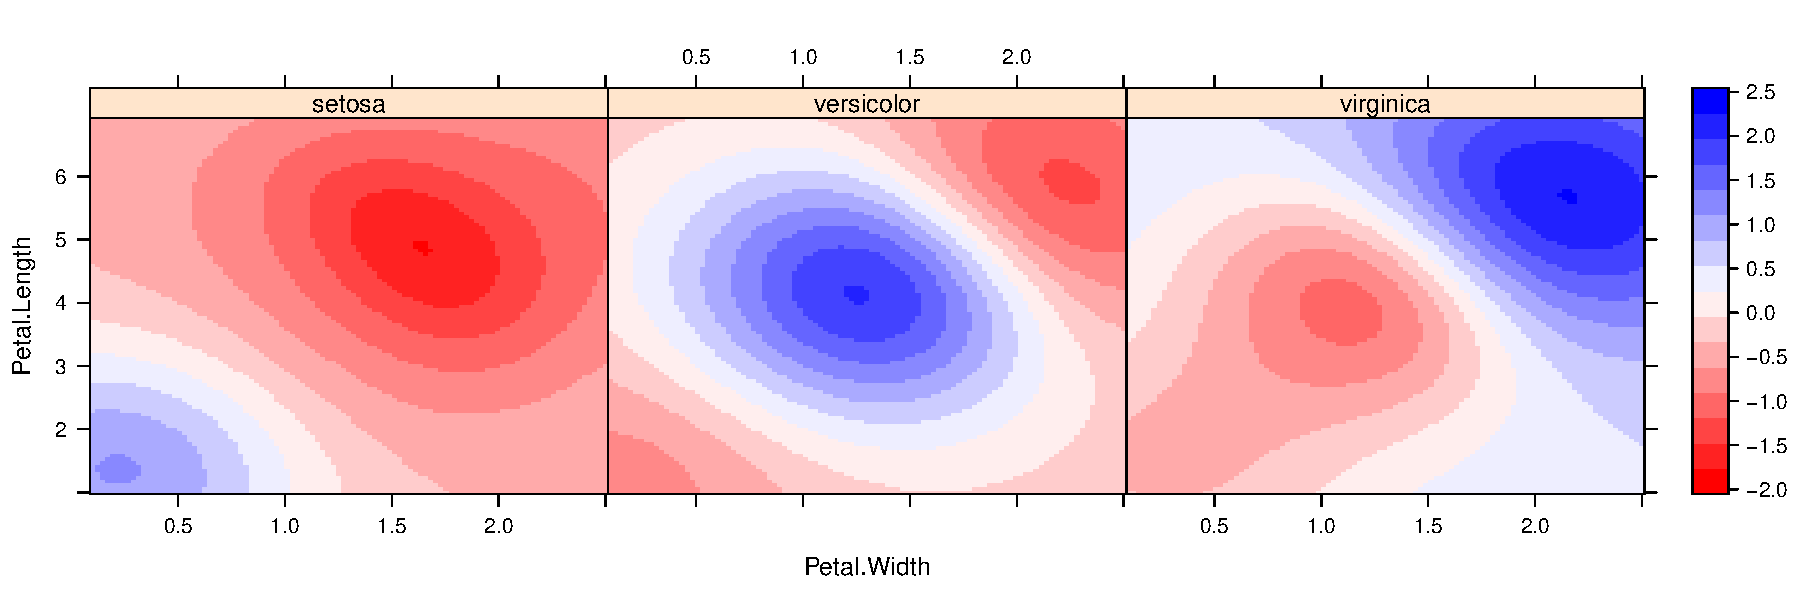
\includegraphics[width=1.0\linewidth]{partial_iris_svm}
  \caption{Partial dependence of \code{Species} on \code{Petal.Width} and \code{Petal.Length} for the iris data.}
  \label{fig:partial_iris}
\end{figure}


%%%%%%%%%%%%%%%%%%%%%%%%%%%%%%%%%%%%%%%%%%%%%%%%%%%%%%%%%%%%%%%%%%%%%%%%%%%%%%%%
% User-defined prediction functions
%%%%%%%%%%%%%%%%%%%%%%%%%%%%%%%%%%%%%%%%%%%%%%%%%%%%%%%%%%%%%%%%%%%%%%%%%%%%%%%%
\subsection{User-defined prediction functions}
\label{sec:prediction}

PDPs are essentially just averaged predictions; see, for example, step 1. (c) in Algorithm~\ref{alg:pdp}. Consequently, as pointed out by \citet{goldstein-peeking-2015}, strong interactions can conceal the complexity of the modeled relationship between the response and predictors of interest. This was part of the motivation behind \citeauthor*{goldstein-peeking-2015}'s ICE plot procedure.

With \code{partial} it is possible to replace the mean in step 1. (c) of Algorithm~\ref{alg:pdp} with any other function (e.g., the median or trimmed mean), or obtain PDPs for classification problems on the probability scale. It is even possible to obtain ICE curves. This flexibility is due to the new \code{pred.fun} argument in \code{partial} (starting with \pkg{pdp} version 0.4.0). This argument accepts an optional prediction function that requires two arguments: \code{object} and \code{newdata}. The supplied prediction function must return either a single prediction or a vector of predictions. Returning the mean of all the predictions will result in the traditional PDP. Returning a vector of predictions (i.e., one for each observation) will result in a set of ICE curves. The examples below illustrate.

Using the \code{pred.fun} argument, it is possible to obtain PDPs for classification problems on the probability scale. We just need to write a function that computes the predicted class probability of interest averaged across all observations. The function below can be used with the fitted SVM from the iris example of Section~\ref{sec:classification} to extract the average predicted probability of belonging to the \code{Setosa} class.
\begin{example}
pred.prob <- function(object, newdata) {  # see ?predict.svm
  pred <- predict(object, newdata, probability = TRUE)
  prob.setosa <- attr(pred, which = "probabilities")[, "setosa"]
  mean(prob.setosa)
}
\end{example}
Next, we simply pass this function via the \code{pred.fun} argument in the call to \code{partial}. The following chunk of code construct PDPs for \code{Petal.Width} and \code{Petal.Length} on the probability scale. The results are displayed in Figure~\ref{fig:partial_iris_prob}.
\begin{example}
# PDPs for Petal.Width and Petal.Length on the probability scale
pdp.pw <- partial(iris.svm, pred.var = "Petal.Width", pred.fun = pred.prob,
                  plot = TRUE)
pdp.pl <- partial(iris.svm, pred.var = "Petal.Length", pred.fun = pred.prob,
                  plot = TRUE)
pdp.pw.pl <- partial(iris.svm, pred.var = c("Petal.Width", "Petal.Length"),
                     pred.fun = pred.prob, plot = TRUE)

# Figure 8
grid.arrange(pdp.pw, pdp.pl, pdp.pw.pl, ncol = 3)
\end{example}

\begin{figure}[!htbp]
  \centering
  \includegraphics[width=1.0\linewidth]{partial_iris_svm_prob}
  \caption{Partial dependence of \code{Species} on \code{Petal.Width} and \code{Petal.Length} plotted on the probability scale; in this case, the probability of belonging to the setosa species.}
  \label{fig:partial_iris_prob}
\end{figure}

For regression problems, the default prediction function is essentially
\begin{example}
pred.fun <- function(object, newdata) {
  mean(predict(object, newdata), na.rm = TRUE)
}
\end{example}
This corresponds to step step 1. (c) in Algorithm~\ref{alg:pdp}. Suppose we would like ICE curves instead. To accomplish this we simply need to pass a prediction function that returns a vector of predictions, one for each observation in \code{newdata}. The code snippet below illustrates this for the Boston housing example using the predictor \code{rm}. The result is displayed in Figure~\ref{fig:ice_boston}. \strong{Note:} when the function supplied to \code{pred.fun} returns multiple predictions, the data frame returned by \code{partial} includes an additional column, \code{yhat.id}, that indicates which curve a point belongs to; in the following code chunk, there will be one curve for each observation in \code{boston}.
\begin{example}
# Use partial to obtain ICE curves
pred.ice <- function(object, newdata) predict(object, newdata)
age.ice <- partial(boston.rf, pred.var = "age", pred.fun = pred.ice)

# Figure 9
plotPartial(age.ice, rug = TRUE, train = boston, alpha = 0.3)
\end{example}
\begin{figure}[!htbp]
  \centering
  \includegraphics[width=0.8\linewidth]{ice_boston}
  \caption{ICE curves depicting the relationship between \code{cmedv} and \code{rm} for the Boston housing example. Each curve corresponds to a different observation.}
  \label{fig:ice_boston}
\end{figure}

The curves in Figure~\ref{fig:ice_boston} indicate some heterogeneity in the fitted model (i.e., some of the curves depict the opposite relationship). Such heterogeneity can be easier to spot using c-ICE curves; see Equation (4) on page 49 of \citet{goldstein-peeking-2015}. Using \CRANpkg{dplyr} \citep{dplyr-pkg}, it is rather straightforward to post-process the output from \code{partial} to obtain c-ICE curves (similar to the construction of \dfn{raw change scores} \citep[pg. 130]{fitzmaurice-2011-applied} for longitudinal data). This is shown below.
\begin{example}
# Post-process rm.ice to obtain c-ICE curves
library(dplyr)  # for group_by and mutate functions
rm.ice <- rm.ice %>%
  group_by(yhat.id) %>%
  mutate(yhat.centered = yhat - first(yhat))
\end{example}

Since the PDP is just the average of the corresponding ICE curves, it is quite simple to display both on the same plot. This can be accomplished by using the \code{stat\_summary} function from the \pkg{ggplot2} package to average the ICE curves together. The code snippet below plots the ICE curves and c-ICE curves, along with their averages, for the predictor \code{rm} in the Boston housing example. The results are displayed in Figure~\ref{fig:ice_cice_boston}.
\begin{example}
# ICE curves with their average
p1 <- ggplot(rm.ice, aes(rm, yhat)) +
  geom_line(aes(group = yhat.id), alpha = 0.2) +
  stat_summary(fun.y = mean, geom = "line", col = "red", size = 1)

# c-ICE curves with their average
p2 <- ggplot(rm.ice, aes(rm, yhat.centered)) +
  geom_line(aes(group = yhat.id), alpha = 0.2) +
  stat_summary(fun.y = mean, geom = "line", col = "red", size = 1)

# Figure 10
grid.arrange(p1, p2, ncol = 2)
\end{example}
\begin{figure}[!htbp]
  \centering
  \includegraphics[width=1.0\linewidth]{ice_cice_boston}
  \caption{ICE curves (black curves) and their average (red curve) depicting the relationship between \code{cmedv} and \code{rm} for the Boston housing example. \textit{Left}: Uncentered (here the red curve is just the traditional PDP). \textit{Right}: Centered.}
  \label{fig:ice_cice_boston}
\end{figure}


%%%%%%%%%%%%%%%%%%%%%%%%%%%%%%%%%%%%%%%%%%%%%%%%%%%%%%%%%%%%%%%%%%%%%%%%%%%%%%%%
% Using partial with xgboost
%%%%%%%%%%%%%%%%%%%%%%%%%%%%%%%%%%%%%%%%%%%%%%%%%%%%%%%%%%%%%%%%%%%%%%%%%%%%%%%%
\subsection{Using partial with the XGBoost library}
\label{sec:xgboost}

To round out our discussion, we provide one last example using a recently popular (and successful!) machine learning tool. XGBoost, short for eXtreme Gradient Boosting, is a popular library providing optimized distributed gradient boosting that is specifically designed to be highly efficient, flexible and portable. The associated R package \pkg{xgboost} has been used to win a number of \href{https://www.kaggle.com/}{Kaggle competitions}. It has been shown to be many times faster than the well-known \pkg{gbm} package. However, unlike \pkg{gbm}, \pkg{xgboost} does not have built-in functions for constructing PDPs. Fortunately, the \pkg{pdp} package can be used to fill this gap.

For illustration, we return to the Boston housing example. The code chunk below uses \pkg{caret} to tune an \pkg{xgboost} model using 10-fold cross-validation. (After loading \pkg{caret}, use \code{getModelInfo("xgbTree")} for information on tuning \pkg{xgboost} models.) \strong{Warning:} The following code chunk may take a few minutes to run.
\begin{example}
# Tune an XGBoost model using 10-fold cross-validation
library(caret)  # functions related to classification and regression training
set.seed(202)  # for reproducibility
boston.xgb <- train(x = data.matrix(subset(boston, select = -cmedv)),
                    y = boston$cmedv, method = "xgbTree", metric = "Rsquared",
                    trControl = trainControl(method = "cv", number = 10),
                    tuneLength = 10)
\end{example}
The optimal model had a cross-validated $R^2$ of $0.902$ (use \code{print(boston.xgb\$bestTune)} to view the optimum tuning parameters). The next snippet of code computes the partial dependence of \code{cmedv} on both \code{rm} and \code{lstat}, individually and together. The results are displayed in Figure~\ref{fig:boston_xgb}.
\begin{example}
# PDPs for lstat and rm
pdp.lstat <- partial(boston.xgb, pred.var = "lstat", plot = TRUE, rug = TRUE)
pdp.rm <- partial(boston.xgb, pred.var = "rm", plot = TRUE, rug = TRUE)
pdp.lstat.rm <- partial(boston.xgb, pred.var = c("lstat", "rm"),
                        plot = TRUE, chull = TRUE)

# Figure 11
grid.arrange(pdp.lstat, pdp.rm, pdp.lstat.rm, ncol = 3)
\end{example}
\begin{figure}[!htbp]
  \centering
  \includegraphics[width=1.0\linewidth]{boston_xgb}
  \caption{PDPs for the top two most important variables in the Boston housing data using \pkg{xgboost}. Compare this to the random forest results displayed in Figures~\ref{fig:partial_extrap}-\ref{fig:partial_manual}.}
  \label{fig:boston_xgb}
\end{figure}
%\code{nrounds = 100}, \code{max\_depth = 5}, \code{eta = 0.3}, \code{gamma = 0}, \code{colsample\_bytree = 0.8}, \code{min\_child\_weight = 1}, and \code{subsample = 0.9444444}

The \code{train} function creates objects of class \code{"train"}, whereas the \code{xgboost} function creates objects of class \code{"xgb.Booster"}. Since \code{train} defaults to storing a copy of the training data as part of the \code{"train"} object, there is no need to supply it in the call to \code{partial} in this example. However, this is not the case when using the \pkg{xgboost} package directly. To illustrate, we fit the same model using the \code{xgboost} function with the tuning parameters found previously using \pkg{caret}.
\begin{example}
library(xgboost)  # for xgboost function
set.seed(203)  # for reproducibility
boston.xgb <- xgboost(data = data.matrix(subset(boston, select = -cmedv)),
                      label = boston$cmedv, objective = "reg:linear",
                      nrounds = 100, max_depth = 5, eta = 0.3, gamma = 0,
                      colsample_bytree = 0.8, min_child_weight = 1,
                      subsample = 0.9444444)
\end{example}
To use \code{partial} with \code{"xgb.Booster"} objects, we need to supply the original training data (minus the response) in the call to \code{partial}. The following snippet of code computes the partial dependence of \code{cmedv} on \code{rm} (plot not shown). (Make sure you are using version 0.6-0 or later of \pkg{xgboost}: \url{https://github.com/dmlc/xgboost/tree/master/R-package}.) \strong{Note:} while \code{xgboost} requires the training data to be an object of class \code{"matrix"}, \code{"dgCMatrix"}, or \code{"xgb.DMatrix"}, \code{partial} requires a \code{"data.frame"} that does not contain the response column.
\begin{example}
partial(boston.xgb, pred.var = "rm", plot = TRUE, rug = TRUE,
        train = subset(boston, select = -cmedv))
\end{example}


%%%%%%%%%%%%%%%%%%%%%%%%%%%%%%%%%%%%%%%%%%%%%%%%%%%%%%%%%%%%%%%%%%%%%%%%%%%%%%%%
% Summary
%%%%%%%%%%%%%%%%%%%%%%%%%%%%%%%%%%%%%%%%%%%%%%%%%%%%%%%%%%%%%%%%%%%%%%%%%%%%%%%%
\section{Summary}

PDPs can be used to graphically examine the dependence of the response on low cardinality subsets of the features, accounting for the average effect of the other predictors. In this paper, we showed how to construct PDPs for various types of black box models in R using the \pkg{pdp} package. We also briefly discussed related approaches available in other R packages. Suggestions to avoid extrapolation and high execution times were discussed and demonstrated via examples.

In terms of future development, \pkg{pdp} can be expanded in a number of ways. For example, it would be useful to have the ability to construct PDPs for black box survival models---like conditional random forests with censored response. It would also be worthwhile to implement the partial dependence-based $H$-statistic \citep{friedman-2008-predictive} for assessing the strength of interaction between predictors.


%%%%%%%%%%%%%%%%%%%%%%%%%%%%%%%%%%%%%%%%%%%%%%%%%%%%%%%%%%%%%%%%%%%%%%%%%%%%%%%%
% Summary
%%%%%%%%%%%%%%%%%%%%%%%%%%%%%%%%%%%%%%%%%%%%%%%%%%%%%%%%%%%%%%%%%%%%%%%%%%%%%%%%
\section{Acknowledgments}

TBD.


%%%%%%%%%%%%%%%%%%%%%%%%%%%%%%%%%%%%%%%%%%%%%%%%%%%%%%%%%%%%%%%%%%%%%%%%%%%%%%%%
% Back matter
%%%%%%%%%%%%%%%%%%%%%%%%%%%%%%%%%%%%%%%%%%%%%%%%%%%%%%%%%%%%%%%%%%%%%%%%%%%%%%%%

\bibliography{greenwell}

\address{Brandon M. Greenwell\\
  Infoscitex Corporation\\
  4027 Colonel Glenn Highway\\
  Suite 210\\
  Dayton, OH 45431-1672\\
  United States of America\\}
\email{greenwell.brandon@gmail.com}
